\documentclass[12pt]{article}

\title{\vspace{-3em}PHYS 202a HW 5}
\author{Michael Cardiff}
\date{\today}

\usepackage{amssymb,amsthm,bm,physics,slashed}

\usepackage{caption,enumitem,float,geometry,graphicx,tikz}
\usepackage{tikz-feynhand}

\graphicspath{ {./figs/} }
\captionsetup{labelfont=bf}
\geometry{margin=1in}

\renewcommand{\L}{\mathcal{L}}
\renewcommand{\H}{\mathcal{H}}
\newcommand{\D}{\partial}
\newcommand{\veps}{\varepsilon}
\newcommand{\circled}[1]{\tikz[baseline=(char.base)]{
    \node[shape=circle,draw,inner sep=2pt](char){#1};}}

\setlength{\feynhandtopsep}{0.7mm}

\begin{document}
\maketitle
\section{Maxwell's Equations}

\section{Real Scalars}
Note the interaction Lagrangian is:
\begin{align*}
  \L_I=-\frac12g\chi^2\phi
\end{align*}

\subsection{Feynman Rule}
We need to find the following Feynman rule:
\begin{align*}
  \begin{tikzpicture}[baseline=-0.15cm]
    \begin{feynhand}
      \vertex (a) at (0,0);
      \vertex (c1) at (-1,-1) {$\chi$};
      \vertex (c2) at (-1, 1) {$\chi$};
      \vertex (b) at (1.5,0)  {$\phi$};
      \propag (a) to (c1);
      \propag (a) to (c2);
      \propag[bos] (a) to (b);
    \end{feynhand}
  \end{tikzpicture}
  = -i\mathcal{M}
\end{align*}
Where the matrix element is given by:
\begin{align*}
  \mel{p_3}{i\L_I}{p_1p_2}=N_1N_2N_3e^{-i(p_1+p_2-p_3)\vdot x}(-i\mathcal{M})
\end{align*}
This then boils down to finding the combinatoric factor for the following expectation value:
\begin{align*}
  \mel**{p_3}{-i\frac{g}{2}\chi^2\phi}{p_1p_2}=
  \mel**{\phi(p_3)}{-i\frac{g}{2}\chi^2\phi}{\chi(p_1)\chi(p_2)}
\end{align*}
We find the combinatoric factor from:
\begin{itemize}
\item 2 Ways of annihilating $\chi(p_1)$ and $\chi(p_2)$
\item 1 way of creating $\phi(p_3)$
\end{itemize}
So overall, we have:
\begin{align*}
  \mel{p_3}{i\L_I}{p_1p_2}&=N_1N_2N_3e^{-i(p_1+p_2-p_3)\vdot x}\times
  \overbrace{\qty(-i\frac{2}{2}g)}^{-i\mathcal{M}}\\
  \implies i\mathcal{M}&=ig
\end{align*}
Hence we have the Feynman rule:
\begin{align*}
  \boxed{
    \begin{tikzpicture}[baseline=-0.15cm]
      \begin{feynhand}
        \vertex (a) at (0,0);
        \vertex (c1) at (-1,-1) {$\chi$};
        \vertex (c2) at (-1, 1) {$\chi$};
        \vertex (b) at (1.5,0)  {$\phi$};
        \propag (a) to (c1);
        \propag (a) to (c2);
        \propag[bos] (a) to (b);
      \end{feynhand}
    \end{tikzpicture}
    = -ig}
\end{align*}
Recall we also have the two propagators, simply given by the position space Feynman propagator:
\begin{align*}
  \begin{tikzpicture}[baseline=-0.1cm]
    \begin{feynhand}
      \vertex (a) at (0,0);
      \vertex (b) at (1.5,0);
      \propag (a) to [edge label=$\chi$] (b);
    \end{feynhand}
  \end{tikzpicture}
  =\int\frac{\dd[4]{q}}{(2\pi)^4}
  \frac{i}{q^2-m^2_{\chi}+i\veps}
  \\
  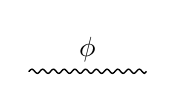
\begin{tikzpicture}[baseline=-0.1cm]
    \begin{feynhand}
      \vertex (a) at (0,0);
      \vertex (b) at (1.5,0);
      \propag[bos] (a) to [edge label=$\phi$] (b);
    \end{feynhand}
  \end{tikzpicture}
  =\int\frac{\dd[4]{q}}{(2\pi)^4}
  \frac{i}{q^2-m^2_{\phi}+i\veps}
\end{align*}

\subsection{Tree-Level Scattering Amplitude}
The process we are looking into is:
\begin{align*}
  \chi+\chi\to\chi+\chi
\end{align*}
Which corresponds to 4 external vertices. Since $\chi$ is a real field, it is its own anti-particle, so we will have an $s$-channel like diagram:
\begin{figure}[H]
  \centering
  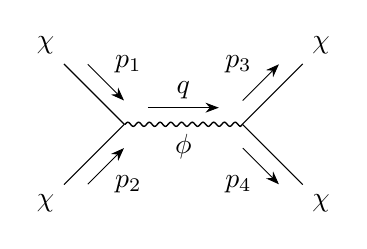
\begin{tikzpicture}
    \begin{feynhand}
      \vertex (a) at (0,0);
      \vertex (c1) at (-1, 1) {$\chi$};
      \vertex (c2) at (-1,-1) {$\chi$};
      \vertex (c3) at (2.5, 1) {$\chi$};
      \vertex (c4) at (2.5, -1) {$\chi$};
      \vertex (b) at (1.5,0);
      \propag [mom={$p_1$}] (c1) to (a);
      \propag [mom'={$p_2$}] (c2) to (a);
      \propag [mom={$p_3$}] (b) to (c3);
      \propag [mom'={$p_4$}] (b) to (c4);
      \propag [bos, mom={$q$}] (a) to [edge label'=$\phi$] (b);
    \end{feynhand}
  \end{tikzpicture}
  \caption{One Possible Diagram, $s$-channel}
  \label{fig:s}
\end{figure}
Then we can have the two particles exchange a $\phi$, this can happen in 2 different ways, $t$ or $u$ channel, giving the following 2 diagrams:
\begin{figure}[H]
  \centering
  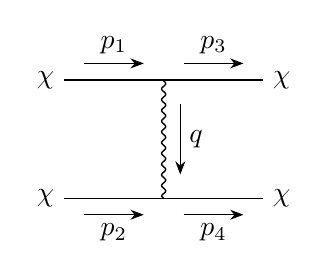
\begin{tikzpicture}
    \begin{feynhand}
      % phi
      \vertex (p1) at (0,0.75);
      \vertex (p2) at (0,-0.75);
      % chis
      \vertex (c1) at (-1.5, 0.75) {$\chi$};
      \vertex (c2) at (-1.5,-0.75) {$\chi$};
      \vertex (c3) at (1.5, 0.75) {$\chi$};
      \vertex (c4) at (1.5, -0.75) {$\chi$};
      % connections
      \propag [bos, mom=$q$] (p1) to (p2);
      \propag [mom=$p_1$] (c1) to (p1);
      \propag [mom=$p_3$] (p1) to (c3);
      \propag [mom'=$p_2$] (c2) to (p2);
      \propag [mom'=$p_4$] (p2) to (c4);
    \end{feynhand}
  \end{tikzpicture}
    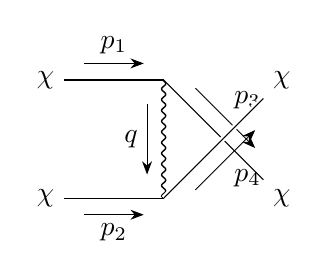
\begin{tikzpicture}
    \begin{feynhand}
      % phi
      \vertex (p1) at (0,0.75);
      \vertex (p2) at (0,-0.75);
      % chis
      \vertex (c1) at (-1.5, 0.75) {$\chi$};
      \vertex (c2) at (-1.5,-0.75) {$\chi$};
      \vertex (c3) at (1.5, -0.75) {$\chi$};
      \vertex (c4) at (1.5, 0.75) {$\chi$};
      % connections
      \propag [bos, mom'=$q$] (p1) to (p2);
      \propag [mom=$p_1$] (c1) to (p1);
      \propag [mom=$p_3$] (p1) to (c3);
      \propag [mom'=$p_2$] (c2) to (p2);
      \propag [top, mom'=$p_4$] (p2) to (c4);
    \end{feynhand}
  \end{tikzpicture}
  \caption{Two Possible Diagrams, $t,u$-channel respectively}
  \label{fig:tu}
\end{figure}
We can calculate the matrix elements $\mathcal{M}_{fi}^{(s,t,u)}$ using the Feynman rules in Section 5.6 of D\&S. First we find $\mathcal{M}_{fi}^{(s)}$ using the diagram in figure \ref{fig:s}:
\begin{enumerate}
\item We have 2 vertices, so we start with:
  \begin{align*}
    (-ig)(-ig)
  \end{align*}
\item Next, we have a factor of the propagator:
  \begin{align*}
    (-ig)(-ig)\int\frac{\dd[4]{q}}{(2\pi)^4}\frac{i}{q^2-m_\phi^2+i\veps}
  \end{align*}
\item We then impose momentum conservation at each vertex using a $\delta$:
  \begin{align}
    \label{eq:sint}
    \circled{1}:=
    (-ig)(-ig)\int\frac{\dd[4]{q}}{(2\pi)^4}
    \frac{i(2\pi)^8\delta^{(4)}(p_1+p_2-q)\delta^{(4)}(q-p_3-p_4)}
    {q^2-m_\phi^2+i\veps}
  \end{align}
\end{enumerate}

We can then evaluate the $\delta$ function integral in eq \eqref{eq:sint} to find:
\begin{align*}
  \circled{1}=
  -i(2\pi)^4\delta^{(4)}(p_1+p_2-p_3-p_4)\frac{g^2}{(p_1+p_2)^2-m_\phi^2+i\veps}
\end{align*}
Note that this is:
\begin{align*}
  -i(2\pi)^4\delta^{(4)}(\text{momentum conservation})\mathcal{M}_{fi}
\end{align*}
So we can identify:
\begin{align*}
  \mathcal{M}^{(s)}_{fi}=\frac{g^2}{(p_1+p_2)^2-m^2_\phi+i\veps}
\end{align*}

The t and u-channel diagrams only have a different step 3, as each vertex has a different momenta:
\begin{gather*}
  q^{(t)}=p_1-p_3=p_4-p_2\\
  q^{(u)}=p_1-p_4=p_3-p_2
\end{gather*}
So the momen
tum-conserving $\delta$ functions are:
\begin{align*}
  t\text{-channel: }
  (2\pi)^4\delta^{(4)}(p_1-p_3-q)(2\pi)^4\delta^{(4)}(q-p_3+p_2)\\
  u\text{-channel: }
  (2\pi)^4\delta^{(4)}(p_1-p_4-q)(2\pi)^4\delta^{(4)}(q-p_4+p_2)
\end{align*}
We then get The following integrals:
\begin{align*}
  \circled{2}&:= (-ig)(-ig)\int\frac{\dd[4]{q}}{(2\pi)^4}
  \frac{i(2\pi)^8\delta^{(4)}(p_1-p_3-q)\delta^{(4)}(q-p_3+p_2)}
  {q^2-m_\phi^2+i\veps}\\
  \circled{3}&:= (-ig)(-ig)\int\frac{\dd[4]{q}}{(2\pi)^4}
  \frac{i(2\pi)^8\delta^{(4)}(p_1-p_4-q)\delta^{(4)}(q-p_4+p_2)}
  {q^2-m_\phi^2+i\veps}
\end{align*}
We can then identify each of the other $\mathcal{M}_{fi}$s by evaluating the integrals $\circled{1}$ and $\circled{2}$:
\begin{align*}
  \circled{2} = -i(2\pi)^4\delta^{(4)}(p_1-p_3-p_4+p_2)
  \frac{g^2}{(p_1-p_3)^2-m^2_\phi+i\veps}
  \\
  \circled{3} = -i(2\pi)^4\delta^{(4)}(p_1-p_4-p_3+p_2)
  \frac{g^2}{(p_1-p_4)^2-m^2_\phi+i\veps}
\end{align*}
We can then summarize each of the matrix elements as invariant amplitudes:
\begin{equation}
  \label{eq:mels}
  \boxed{\begin{aligned}
      i\mathcal{M}^{(s)}_{fi}&=\frac{ig^2}{(p_1+p_2)^2-m^2_\phi+i\veps}\\
      i\mathcal{M}^{(t)}_{fi}&=\frac{ig^2}{(p_1-p_3)^2-m^2_\phi+i\veps}\\
      i\mathcal{M}^{(u)}_{fi}&=\frac{ig^2}{(p_1-p_4)^2-m^2_\phi+i\veps}
  \end{aligned}}
\end{equation}

\subsection{One Loop Diagrams for $\phi$ scattering}
We are considering scattering of $\phi$ particles:
\begin{align*}
  \phi+\phi\to\phi+\phi
\end{align*}
Which have no tree-level diagrams, we only have the following 3 'box' diagrams, one that looks like a $t$ channel, one that looks like a $u$ channel and a $t$ channel with the internal momenta swapped:
\begin{figure}[H]
  \centering
  % t channel
  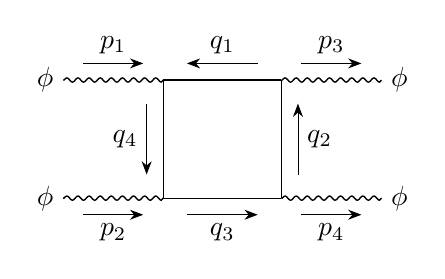
\begin{tikzpicture}
    \begin{feynhand}
      % phis
      \vertex (p1) at (-0.5,0.5) {$\phi$}; \vertex (p2) at (-0.5,-1) {$\phi$};
      \vertex (p3) at (   4,0.5) {$\phi$}; \vertex (p4) at (   4,-1) {$\phi$};
      % chis
      \vertex (c1) at (1, 0.5); \vertex (c2) at (2.5, 0.5);
      \vertex (c3) at (1,-1); \vertex (c4) at (2.5,-1);
      % external connections
      \propag [bos, mom=$p_1$] (p1) to (c1);
      \propag [bos, mom'=$p_2$] (p2) to (c3);
      \propag [bos, mom=$p_3$] (c2) to (p3);
      \propag [bos, mom'=$p_4$] (c4) to (p4);
      % internal connections
      \propag [revmom=$q_1$] (c1) to (c2); \propag [revmom=$q_2$] (c2) to (c4);
      \propag [revmom=$q_3$] (c4) to (c3); \propag [revmom=$q_4$] (c3) to (c1);
    \end{feynhand}
  \end{tikzpicture}
  % u channel
  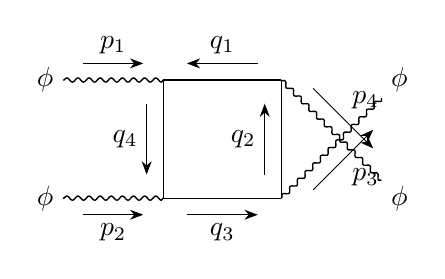
\begin{tikzpicture}
    \begin{feynhand}
      % phis
      \vertex (p1) at (-0.5,0.5) {$\phi$}; \vertex (p2) at (-0.5,-1) {$\phi$};
      \vertex (p3) at (4   ,0.5) {$\phi$}; \vertex (p4) at (   4,-1) {$\phi$};
      % chis
      \vertex (c1) at (1, 0.5); \vertex (c2) at (2.5, 0.5);
      \vertex (c3) at (1,  -1); \vertex (c4) at (2.5,  -1);
      % external connections
      \propag [bos, mom=$p_1$] (p1) to (c1);
      \propag [bos, mom'=$p_2$] (p2) to (c3);
      \propag [bos, mom'=$p_3$] (c4) to (p3);
      \propag [bos, mom=$p_4$] (c2) to (p4);
      % internal connections
      \propag [revmom=$q_1$] (c1) to (c2); \propag [revmom'=$q_2$] (c2) to (c4);
      \propag [revmom=$q_3$] (c4) to (c3); \propag [revmom=$q_4$] (c3) to (c1);
    \end{feynhand}
  \end{tikzpicture}
  \\
  % t channel swap
  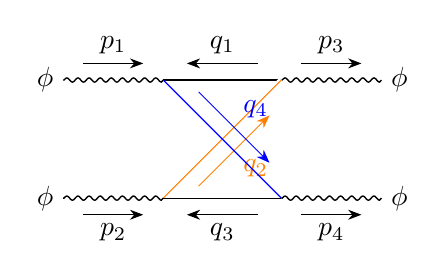
\begin{tikzpicture}
    \begin{feynhand}
      % phis
      \vertex (p1) at (-0.5,0.5) {$\phi$}; \vertex (p2) at (-0.5,-1) {$\phi$};
      \vertex (p3) at (4   ,0.5) {$\phi$}; \vertex (p4) at (   4,-1) {$\phi$};
      % chis
      \vertex (c1) at (1, 0.5); \vertex (c2) at (2.5, 0.5);
      \vertex (c3) at (1,  -1); \vertex (c4) at (2.5,  -1);
      % external connections
      \propag [bos, mom=$p_1$] (p1) to (c1);
      \propag [bos, mom'=$p_2$] (p2) to (c3);
      \propag [bos, mom=$p_3$] (c2) to (p3);
      \propag [bos, mom'=$p_4$] (c4) to (p4);
      % internal connections
      \propag [revmom=$q_1$] (c1) to (c2); 
      \propag [top, orange, revmom={[arrow style=orange] $q_2$}] (c2) to (c3);
      \propag [revmom'=$q_3$] (c3) to (c4); 
      \propag [blue, revmom'={[arrow style=blue] $q_4$}] (c4) to (c1);
    \end{feynhand}
  \end{tikzpicture}
  \caption{Box Diagrams}
  \label{fig:box}
\end{figure}
Note that the bottom diagram is stretched out to make the momentum labelling a bit easier to read

We will start with the diagram on the left, and generalize from there.
\begin{enumerate}
\item Factor of $-ig$ for each vertex:
  \begin{align*}
    (-ig)^4
  \end{align*}
  Then we have 4 internal momenta to integrate over, for now leaving out the $i\veps$ terms
  \begin{align*}
    (-ig)^4&\int\frac{\dd[4]{q_1}\dd[4]{q_2}\dd[4]{q_3}\dd[4]{q_4}}
    {(2\pi)^4(2\pi)^4(2\pi)^4(2\pi)^4}
    \frac{i^4}{(q_1^2-m_\chi^2)(q_2^2-m_\chi^2)(q_3^2-m_\chi^2)(q_4^2-m_\chi^2)}\\
    =(-ig)^4&\int\dd{Q}
    \frac{i^4}{(q_1^2-m_\chi^2+i\veps)(q_2^2-m_\chi^2+i\veps)(q_3^2-m_\chi^2+i\veps)(q_4^2-m_\chi^2+i\veps)}
  \end{align*}
  From here on, the measure of the integral will be called $\dd{Q}$ such that:
  \begin{align*}
    \dd{Q}=\frac{\dd[4]{q_1}\dd[4]{q_2}\dd[4]{q_3}\dd[4]{q_4}}
    {(2\pi)^4(2\pi)^4(2\pi)^4(2\pi)^4}
  \end{align*}
\item Impose momentum conservation at each vertex:
  \begin{align*}
    \circled{1}=(2\pi)^4\delta^{(4)}(p_1-q_1+q_4)\\
    \circled{2}=(2\pi)^4\delta^{(4)}(q_1-p_3-q_2)\\
    \circled{3}=(2\pi)^4\delta^{(4)}(q_3-q_2-p_4)\\
    \circled{4}=(2\pi)^4\delta^{(4)}(q_4-p_2-q_3)
  \end{align*}
  Meaning in total, the basic matrix element is given by:
  \begin{align*}
    (-ig)^4\int\dd{Q}
    \frac{i^4\circled{1}\circled{2}\circled{3}\circled{4}}
    {(q_1^2-m_\chi^2+i\veps)(q_2^2-m_\chi^2+i\veps)(q_3^2-m_\chi^2+i\veps)(q_4^2-m_\chi^2+i\veps)}
  \end{align*}
\end{enumerate}
% We can evaluate some of these integrals, first using $\circled{2}$ to evaluate the $q_1$
% \begin{align*}
%   &(-ig)^4\int\dd{Q}_{\text{no }q_1}i^4(2\pi)^{12}
%   \delta^{(4)}(p_1-p_3-q_2+q_4)
%   \delta^{(4)}(q_3-q_2-p_4)
%   \delta^{(4)}(q_4-p_2-q_3)
% \end{align*}
% This will turn the $q_1$ propagator term into:
% \begin{align*}
%   \frac{1}{q_1^2-m_\chi^2}=\frac{1}{(p_3+q_2)^2-m_\chi^2}
% \end{align*}
% We should then use $\circled{3}$ to evaluate $q_3$
% \begin{align*}
%   &(-ig)^4\int\dd{Q}_{\text{no }q_1,q_3}i^4(2\pi)^{8}
%   \delta^{(4)}(p_1-p_3+(q_4-q_2))
%   \delta^{(4)}(q_4-q_2-p_2-p_4)
% \end{align*}
% Turning the $q_3$ propagator into:
% \begin{align*}
%   \frac{1}{q_3^2-m_\chi^2}=\frac{1}{(q_2+p_4)^2-m_\chi^2}
% \end{align*}
% I am not sure how to go about the specific change of variables here since it is a multidimensional integral, but we can denote $q_4$ by $q+k$ and $q_2$ by $k$ such that $q_4-q_2=q$, and we can have
% \begin{align*}
%   g^4\int\frac{\dd[4]{q}\dd[4]{k}}{(2\pi)^8}(2\pi)^8
%   \delta^{(4)}(p_1-p_3+q)
%   \delta^{(4)}(q-p_2-p_4)
% \end{align*}
% Note this does change the propagator terms as well:
% \begin{align*}
%   \frac{1}{q_2^2-m_\chi^2}&=\frac{1}{k^2-m_\chi^2}\\
%   \frac{1}{q_4^2-m_\chi^2}&=\frac{1}{(q+k)^2-m_\chi^2}
% \end{align*}
% So we can integrate out $q$:
% \begin{align*}
%   g^4\int\frac{\dd[4]{k}}{(2\pi)^4}(2\pi)^4
%   \delta^{(4)}(p_1-p_3+p_2-p_4)
% \end{align*}
The arguments of the delta functions can be solved in terms of 1 single $q$, to get a total momentum conserving delta function then a single integral over $q_1$
\begin{align*}
  q_1&=q_1\\
  q_2&=q_1+p_2\\
  q_3&=q_1+p_1+p_2\\
  q_4&=q_1+p_3
\end{align*}
Giving:
\begin{align*}
  -i(2\pi)^4&\delta^{(4)}(p_1+p_2-p_3-p_4)\\
  &\times\int\frac{\dd[4]{q_1}}{(2\pi)^4}
  \frac{ig^4}{(q_1^2-m_\chi^2)((q_1+p_2)^2-m_\chi^2)
    ((q_1+p_1+p_2)^2-m_\chi^2)((q_1+p_3)^2-m_\chi^2)}
\end{align*}
This gives $\mathcal{M}_{fi}$ for this diagram as:
\begin{align*}
  \mathcal{M}_{fi}^{(1)}=
  \int\frac{\dd[4]{q_1}}{(2\pi)^4}ig^4&
  \frac1{q_1^2-m_\chi^2+i\veps}\frac1{(q_1+p_1+p_2)^2-m_\chi^2+i\veps}\\
  &\times\frac1{(q_1+p_2)^2-m_\chi^2+i\veps}\frac1{(q_1+p_3)^2-m_\chi^2+i\veps}
\end{align*}
The middle diagram simply has $p_4$ and $p_3$ swapped:
\begin{align*}
  \mathcal{M}_{fi}^{(2)}=
  \int \frac{\dd[4]{q_1}}{(2\pi)^4}ig^4&
  \frac1{q_1^2-m_\chi^2+i\veps}\frac1{(q_1+p_1+p_2)^2-m_\chi^2+i\veps}\\
  &\times\frac1{(q_1+p_2)^2-m_\chi^2+i\veps}\frac1{(q_1+p_4)^2-m_\chi^2+i\veps}
\end{align*}
The last diagram on the bottom of fig \ref{fig:box} has the following for momentum conservation:
\begin{align*}
  \circled{1}=(2\pi)^4\delta^{(4)}(p_1-q_1+q_4)\\
  \circled{2}=(2\pi)^4\delta^{(4)}(q_1-p_3-q_2)\\
  \circled{3}=(2\pi)^4\delta^{(4)}(q_3-q_2-p_2)\\
  \circled{4}=(2\pi)^4\delta^{(4)}(q_4-p_4-q_3)
\end{align*}
Which will result in the momenta changing to:
\begin{align*}
    q_1&=q_1\\
    q_2&=p_3-q_1\\
    q_3&=p_2+p_3-q_1\\
    q_4&=p_4+p_2+p_3-q_1
\end{align*}
Giving $\mathcal{M}_{fi}$ as:
\begin{align*}
  \mathcal{M}_{fi}^{(3)}=
  \int \frac{\dd[4]{q_1}}{(2\pi)^4}ig^4&
  \frac1{q_1^2-m_\chi^2+i\veps}\frac1{(p_4+p_2+p_3-q_1)^2-m_\chi^2+i\veps}\\
  &\times\frac1{(p_2+p_3-q_1)^2-m_\chi^2+i\veps}\frac1{(p_3-q_1)^2-m_\chi^2+i\veps}
\end{align*}
The invariant amplitudes are then
\begin{equation}
    \boxed{\begin{aligned}
    i\mathcal{M}_{fi}^{(1)}=
    -\int\frac{\dd[4]{q_1}}{(2\pi)^4}&g^4
    \frac1{q_1^2-m_\chi^2+i\veps}\frac1{(q_1+p_1+p_2)^2-m_\chi^2+i\veps}\\
    &\times\frac1{(q_1+p_2)^2-m_\chi^2+i\veps}\frac1{(q_1+p_3)^2-m_\chi^2+i\veps}\\
    i\mathcal{M}_{fi}^{(2)}=
    -\int\frac{\dd[4]{q_1}}{(2\pi)^4}&g^4
    \frac1{q_1^2-m_\chi^2+i\veps}\frac1{(q_1+p_1+p_2)^2-m_\chi^2+i\veps}\\
    &\times\frac1{(q_1+p_2)^2-m_\chi^2+i\veps}\frac1{(q_1+p_4)^2-m_\chi^2+i\veps}\\
    i\mathcal{M}_{fi}^{(3 )}=
    -\int\frac{\dd[4]{q_1}}{(2\pi)^4}&g^4
    \frac1{q_1^2-m_\chi^2+i\veps}\frac1{(p_4+p_2+p_3-q_1)^2-m_\chi^2+i\veps}\\
    &\times\frac1{(p_2+p_3-q_1)^2-m_\chi^2+i\veps}\frac1{(p_3-q_1)^2-m_\chi^2+i\veps}
    \end{aligned}}
\end{equation}
I believe that is what we need

\section{Complex Scalars}
Recall the Lagrangian 5.51 and its feynman rule:
\begin{align*}
  \L=\frac12\D_\mu a\D^\mu a+\D_\mu\phi^*\D^\mu\phi
  -\frac12m^2a^2-m_\phi^2\phi^*\phi-ga\phi^*\phi
\end{align*}
However, the book mentions that $a$ is massless, I believe the Lagrangian should be:
\begin{align*}
  \L=\frac12\D_\mu a\D^\mu a+\D_\mu\phi^*\D^\mu\phi
  -m_\phi^2\phi^*\phi-ga\phi^*\phi
\end{align*}
The Feynman rule is:
\begin{align*}
  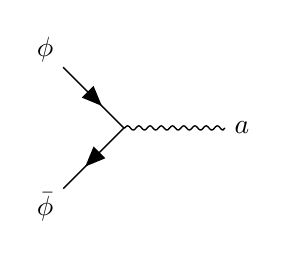
\begin{tikzpicture}[baseline=-0.15cm]
    \begin{feynhand}
      \vertex (a) at (0,0);
      \vertex (c1) at (-1, 1) {$\phi$};
      \vertex (c2) at (-1,-1) {$\bar\phi$};
      \vertex (b) at (1.5,0)  {$a$};
      \propag [antfer] (a) to (c1);
      \propag [fer] (a) to (c2);
      \propag[bos] (a) to (b);
    \end{feynhand}
  \end{tikzpicture}
  = -ig
\end{align*}
Note the arrows are now included to specify the direction of the flow of charge
\subsection{$\phi+\phi\to\phi+\phi$}
Since this process involves no $\bar\phi$, we only have a $t$ and $u$ channel diagram, as charge conservation prevents an $s$-channel diagram:
\begin{figure}[H]
  \centering
  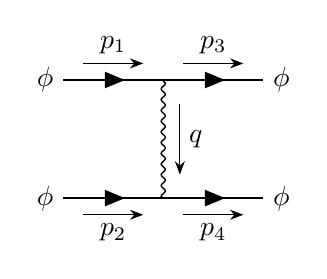
\begin{tikzpicture}
    \begin{feynhand}
      % a
      \vertex (a1) at (0,0.75);
      \vertex (a2) at (0,-0.75);
      % phis
      \vertex (p1) at (-1.5, 0.75) {$\phi$};
      \vertex (p2) at (-1.5,-0.75) {$\phi$};
      \vertex (p3) at (1.5, 0.75) {$\phi$};
      \vertex (p4) at (1.5, -0.75) {$\phi$};
      % connections
      \propag [bos, mom=$q$] (a1) to (a2);
      \propag [fer, mom=$p_1$] (p1) to (a1);
      \propag [fer, mom=$p_3$] (a1) to (p3);
      \propag [fer, mom'=$p_2$] (p2) to (a2);
      \propag [fer, mom'=$p_4$] (a2) to (p4);
    \end{feynhand}
  \end{tikzpicture}
  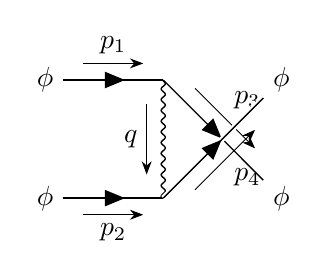
\begin{tikzpicture}
    \begin{feynhand}
      % a
      \vertex (a1) at (0,0.75);
      \vertex (a2) at (0,-0.75);
      % phis
      \vertex (p1) at (-1.5, 0.75) {$\phi$};
      \vertex (p2) at (-1.5,-0.75) {$\phi$};
      \vertex (p3) at (1.5, -0.75) {$\phi$};
      \vertex (p4) at (1.5, 0.75) {$\phi$};
      % connections
      \propag [bos, mom'=$q$] (a1) to (a2);
      \propag [fer, mom=$p_1$] (p1) to (a1);
      \propag [fer, mom=$p_3$] (a1) to (p3);
      \propag [fer, mom'=$p_2$] (p2) to (a2);
      \propag [fer, top, mom'=$p_4$] (a2) to (p4);
    \end{feynhand}
  \end{tikzpicture}
  \caption{Possible Diagrams for $\phi$ scattering}
  \label{fig:tucharge}
\end{figure}

The Matrix Element for these from earlier still holds:
\begin{align*}
  \mathcal{M}^{(t)}_{fi}=
  \frac{g^2}{(p_1-p_3)^2+i\veps}
\end{align*}
The only difference is that the mass of the force carrier is now $0$, so we only have the momentum and $i\veps$.

The $u$-channel is also of this form:
\begin{align*}
  \mathcal{M}^{(u)}_{fi}=
  \frac{g^2}{(p_1-p_3)^2+i\veps}
\end{align*}
So the tree level invariant amplitude is:
\begin{align}
  \boxed{i\mathcal{M}^{(tot)}=
  i\qty(\frac{g^2}{(p_1-p_3)^2+i\veps}+\frac{g^2}{(p_1-p_3)^2+i\veps})}
\end{align}

\subsection{$\phi+\bar\phi\to\phi+\bar\phi$}
Here we have two diagrams, an $s$ channel and $t$ channel:
\begin{figure}[H]
  \centering
    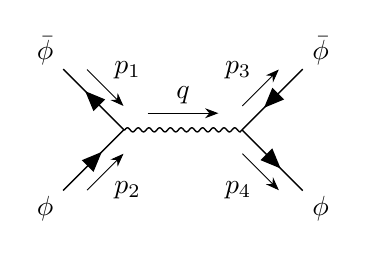
\begin{tikzpicture}
    \begin{feynhand}
      \vertex (a) at (0,0);
      \vertex (p1) at (-1, 1) {$\bar\phi$};
      \vertex (p2) at (-1,-1) {$\phi$};
      \vertex (p3) at (2.5, 1) {$\bar\phi$};
      \vertex (p4) at (2.5, -1) {$\phi$};
      \vertex (b) at (1.5,0);
      \propag [antfer, mom={$p_1$}] (p1) to (a);
      \propag [fer, mom'={$p_2$}] (p2) to (a);
      \propag [antfer, mom={$p_3$}] (b) to (p3);
      \propag [fer, mom'={$p_4$}] (b) to (p4);
      \propag [bos, mom={$q$}] (a) to (b);
    \end{feynhand}
  \end{tikzpicture}
  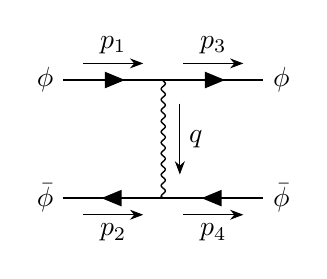
\begin{tikzpicture}
    \begin{feynhand}
      % a
      \vertex (a1) at (0,0.75);
      \vertex (a2) at (0,-0.75);
      % phis
      \vertex (p1) at (-1.5, 0.75) {$\phi$};
      \vertex (p2) at (-1.5,-0.75) {$\bar\phi$};
      \vertex (p3) at (1.5, 0.75) {$\phi$};
      \vertex (p4) at (1.5, -0.75) {$\bar\phi$};
      % connections
      \propag [bos, mom=$q$] (a1) to (a2);
      \propag [fer, mom=$p_1$] (p1) to (a1);
      \propag [fer, mom=$p_3$] (a1) to (p3);
      \propag [antfer, mom'=$p_2$] (p2) to (a2);
      \propag [antfer, mom'=$p_4$] (a2) to (p4);
    \end{feynhand}
  \end{tikzpicture}
  \caption{Diagrams for $\phi+\bar\phi$ to itself}
  \label{fig:ppb}
\end{figure}

The $s$ channel diagram gives the following matrix element, which is the same as before except with a massless force carrier
\begin{align*}
  \mathcal{M}^{(s)}_{fi}=\frac{g^2}{(p_1+p_2)^2+i\veps}
\end{align*}
Then the $t$ channel is exactly the same as before:
\begin{align*}
  \mathcal{M}^{(t)}_{fi}=
  \frac{g^2}{(p_1-p_3)^2+i\veps}
\end{align*}
So the tree level invariant amplitude is:
\begin{align}
  \boxed{i\mathcal{M}^{(tot)}_{fi}=
  i\qty(\frac{g^2}{(p_1+p_2)^2+i\veps}+\frac{g^2}{(p_1-p_3)^2+i\veps})}
\end{align}

\end{document}